\documentclass[12pt]{article}
\usepackage[table]{xcolor}
\usepackage[shortlabels]{enumitem}
\usepackage{tabularx,xltabular}
\usepackage{graphicx}
\usepackage{hyperref}
\usepackage{verbatim}
\usepackage{geometry}
\usepackage{ulem}
\usepackage[official]{eurosym}
\usepackage{tikz}
\usetikzlibrary{arrows,backgrounds,calc,decorations.markings,patterns,3d}
\usepackage{pgfplots}
\pgfplotsset{compat = newest}
\usetikzlibrary{fit}
\newcommand\addvmargin[1]{
\usetikzlibrary{arrows}
\node[fit=(current bounding box),inner ysep=#1,inner xsep=0]{};}
\usepackage{cancel}
\usepackage{fontspec}
\usepackage{array}  
\geometry{a4paper, top=2cm, left=2cm, right=2cm, bottom=2cm, headsep=1cm}
\usepackage{tabu}
\usepackage{pst-node}
\usepackage{colortbl}
\usepackage{array}
\usepackage{german}
\setlength\parindent{0pt}
\newcolumntype{?}{!{\vrule width 1pt}}
\usepackage{makecell}
\renewcommand{\arraystretch}{2.5}
\usepackage{pbox}
\usepackage{amssymb}
\usepackage{amsmath}
\usepackage{booktabs}
\newcolumntype{L}[1]{>{\raggedright\let\newline\\\arraybackslash\hspace{0pt}}m{#1}}
\newcolumntype{C}[1]{>{\centering\let\newline\\\arraybackslash\hspace{0pt}}m{#1}}
\newcolumntype{R}[1]{>{\raggedleft\let\newline\\\arraybackslash\hspace{0pt}}m{#1}}
\begin{document}
\rightline{Datum: 08.06.2023}
\centerline{{\Large Tägliche Übungen}} 
\vspace{1cm}
\noindent \\


\begin{xltabular}{\textwidth}{|C{0.75cm}|X|C{0.75cm}|X|}
\arrayrulecolor{black}\hline
a)&$\begin{aligned}
 b=&-10~ \rightarrow ~ 5 \cdot b + 2=?
\end{aligned}$
&
b)&$\begin{aligned}
 z=&-11~ \rightarrow ~ 1 + z=?
\end{aligned}$
\\\hline
c)&$\begin{aligned}
 x=&-7~ \rightarrow ~ 3 \cdot x - 4 \cdot x=?
\end{aligned}$
&
d)&$\begin{aligned}
 z=&-9~ \rightarrow ~ 1 + z=?
\end{aligned}$
\\\hline
e)&$x+18 = 38$
&
f)&$a+4 = 18$
\\\hline
g)&$x+13 = 31$
&
h)&$a+23 = 21$
\\\hline
i)&$a+37 = 40$
&
j)&$x+19 = 37$
\\\hline
k)&$y+45 = 20$
&
l)&$y-15 = 42$
\\\hline
m)&$a+6 = 2$
&
n)&$x-31 = 9$
\\\hline
o)&$b-4 = 24$
&
p)&$a+40 = 18$
\\\hline
q)&$x+14 = 37$
&
r)&$y+8 = 20$
\\\hline
s)&$x+5 = 43$
&
t)&$a-13 = 43$
\\\hline
u)&$x-5 = 1$
&
v)&$y+2 = 8$
\\\hline
w)&$a-10 = 14$
&
x)&$x+32 = 29$
\\\hline
y)&$x+44 = 32$
&
z)&$b+39 = 49$
\\\hline
\end{xltabular}
\vspace{0.5cm}
\newpage
\rightline{Datum: 08.06.2023}
\centerline{{\large Lösungen Tägliche Übungen}} 
\vspace{0.5cm}

\begin{xltabular}{\textwidth}{|C{0.75cm}|X|C{0.75cm}|X|}
\arrayrulecolor{black}\hline
a)&$\begin{aligned}
\textcolor{red}{b=-10} & \rightarrow\\
5 \cdot b + 2=&5 \cdot \textcolor{red}{(-10)} + 2=-48\\
\end{aligned}$
&
b)&$\begin{aligned}
\textcolor{red}{z=-11} & \rightarrow\\
1 + z=&1 + \textcolor{red}{(-11)}=-10\\
\end{aligned}$
\\\hline
c)&$\begin{aligned}
\textcolor{red}{x=-7} & \rightarrow\\
3 \cdot x - 4 \cdot x=&3 \cdot \textcolor{red}{(-7)} - 4 \cdot \textcolor{red}{(-7)}=7\\
\end{aligned}$
&
d)&$\begin{aligned}
\textcolor{red}{z=-9} & \rightarrow\\
1 + z=&1 + \textcolor{red}{(-9)}=-8\\
\end{aligned}$
\\\hline
e)&\begingroup\setlength{\jot}{-0.03cm}
\tikzstyle{background grid}=[draw, black!15,step=.5cm]
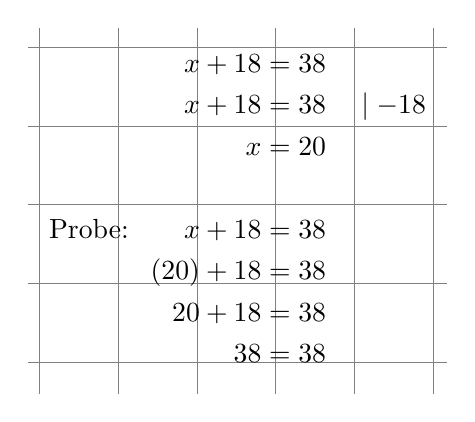
\begin{tikzpicture}[show background grid]
\node[below right] at (0,0.1) {
$\begin{aligned}
x+18  &= 38& &  \\
x + 18 &=38& & \mid - 18\\
x &=20& & 
\\
\\
\mbox{Probe:}\qquad x+18  &= 38& &  \\
\left(20\right)+18  &= 38& &  \\
20+18 &=38& &  \\
38 &=38& &  \\
\end{aligned}$};
\end{tikzpicture}
\endgroup
&
f)&\begingroup\setlength{\jot}{-0.03cm}
\tikzstyle{background grid}=[draw, black!15,step=.5cm]
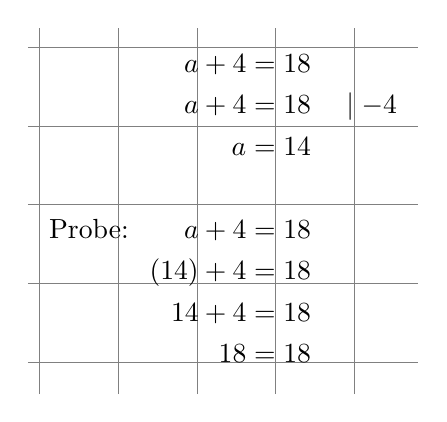
\begin{tikzpicture}[show background grid]
\node[below right] at (0,0.1) {
$\begin{aligned}
a+4  &= 18& &  \\
a + 4 &=18& & \mid - 4\\
a &=14& & 
\\
\\
\mbox{Probe:}\qquad a+4  &= 18& &  \\
\left(14\right)+4  &= 18& &  \\
14+4 &=18& &  \\
18 &=18& &  \\
\end{aligned}$};
\end{tikzpicture}
\endgroup
\\\hline
g)&\begingroup\setlength{\jot}{-0.03cm}
\tikzstyle{background grid}=[draw, black!15,step=.5cm]
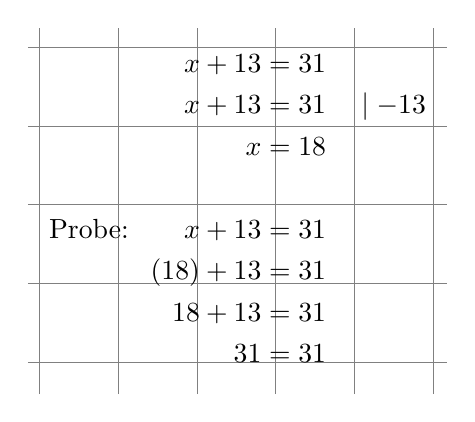
\begin{tikzpicture}[show background grid]
\node[below right] at (0,0.1) {
$\begin{aligned}
x+13  &= 31& &  \\
x + 13 &=31& & \mid - 13\\
x &=18& & 
\\
\\
\mbox{Probe:}\qquad x+13  &= 31& &  \\
\left(18\right)+13  &= 31& &  \\
18+13 &=31& &  \\
31 &=31& &  \\
\end{aligned}$};
\end{tikzpicture}
\endgroup
&
h)&\begingroup\setlength{\jot}{-0.03cm}
\tikzstyle{background grid}=[draw, black!15,step=.5cm]
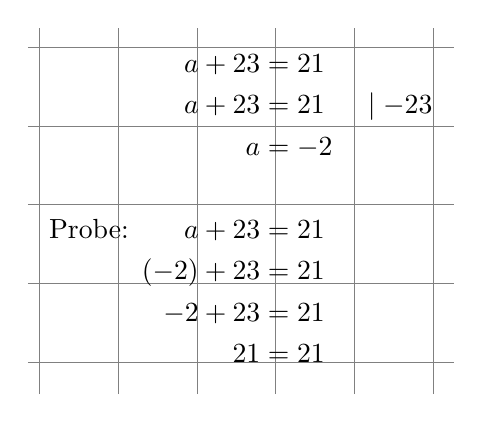
\begin{tikzpicture}[show background grid]
\node[below right] at (0,0.1) {
$\begin{aligned}
a+23  &= 21& &  \\
a + 23 &=21& & \mid - 23\\
a &=-2& & 
\\
\\
\mbox{Probe:}\qquad a+23  &= 21& &  \\
\left(-2\right)+23  &= 21& &  \\
-2+23 &=21& &  \\
21 &=21& &  \\
\end{aligned}$};
\end{tikzpicture}
\endgroup
\\\hline
i)&\begingroup\setlength{\jot}{-0.03cm}
\tikzstyle{background grid}=[draw, black!15,step=.5cm]
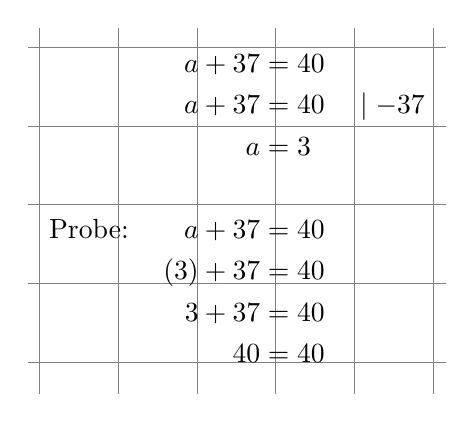
\begin{tikzpicture}[show background grid]
\node[below right] at (0,0.1) {
$\begin{aligned}
a+37  &= 40& &  \\
a + 37 &=40& & \mid - 37\\
a &=3& & 
\\
\\
\mbox{Probe:}\qquad a+37  &= 40& &  \\
\left(3\right)+37  &= 40& &  \\
3+37 &=40& &  \\
40 &=40& &  \\
\end{aligned}$};
\end{tikzpicture}
\endgroup
&
j)&\begingroup\setlength{\jot}{-0.03cm}
\tikzstyle{background grid}=[draw, black!15,step=.5cm]
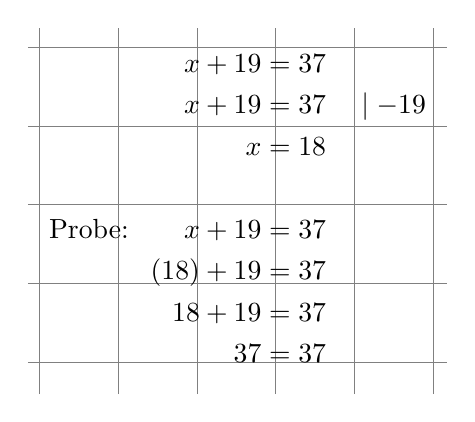
\begin{tikzpicture}[show background grid]
\node[below right] at (0,0.1) {
$\begin{aligned}
x+19  &= 37& &  \\
x + 19 &=37& & \mid - 19\\
x &=18& & 
\\
\\
\mbox{Probe:}\qquad x+19  &= 37& &  \\
\left(18\right)+19  &= 37& &  \\
18+19 &=37& &  \\
37 &=37& &  \\
\end{aligned}$};
\end{tikzpicture}
\endgroup
\\\hline
k)&\begingroup\setlength{\jot}{-0.03cm}
\tikzstyle{background grid}=[draw, black!15,step=.5cm]
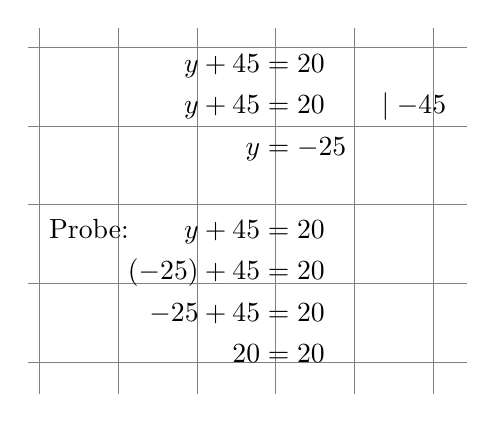
\begin{tikzpicture}[show background grid]
\node[below right] at (0,0.1) {
$\begin{aligned}
y+45  &= 20& &  \\
y + 45 &=20& & \mid - 45\\
y &=-25& & 
\\
\\
\mbox{Probe:}\qquad y+45  &= 20& &  \\
\left(-25\right)+45  &= 20& &  \\
-25+45 &=20& &  \\
20 &=20& &  \\
\end{aligned}$};
\end{tikzpicture}
\endgroup
&
l)&\begingroup\setlength{\jot}{-0.03cm}
\tikzstyle{background grid}=[draw, black!15,step=.5cm]
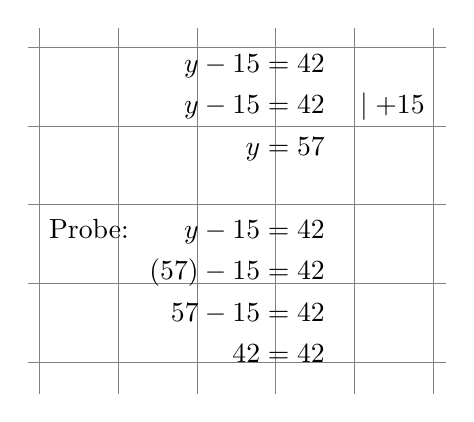
\begin{tikzpicture}[show background grid]
\node[below right] at (0,0.1) {
$\begin{aligned}
y-15  &= 42& &  \\
y - 15 &=42& & \mid + 15\\
y &=57& & 
\\
\\
\mbox{Probe:}\qquad y-15  &= 42& &  \\
\left(57\right)-15  &= 42& &  \\
57-15 &=42& &  \\
42 &=42& &  \\
\end{aligned}$};
\end{tikzpicture}
\endgroup
\\\hline
m)&\begingroup\setlength{\jot}{-0.03cm}
\tikzstyle{background grid}=[draw, black!15,step=.5cm]
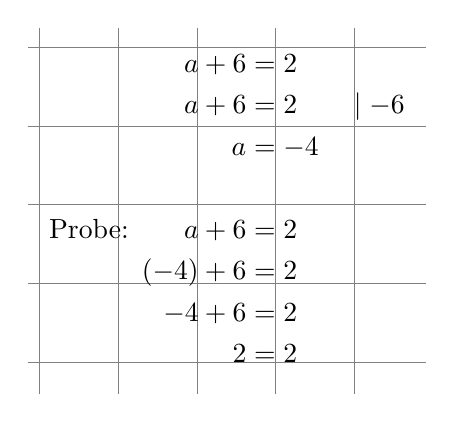
\begin{tikzpicture}[show background grid]
\node[below right] at (0,0.1) {
$\begin{aligned}
a+6  &= 2& &  \\
a + 6 &=2& & \mid - 6\\
a &=-4& & 
\\
\\
\mbox{Probe:}\qquad a+6  &= 2& &  \\
\left(-4\right)+6  &= 2& &  \\
-4+6 &=2& &  \\
2 &=2& &  \\
\end{aligned}$};
\end{tikzpicture}
\endgroup
&
n)&\begingroup\setlength{\jot}{-0.03cm}
\tikzstyle{background grid}=[draw, black!15,step=.5cm]
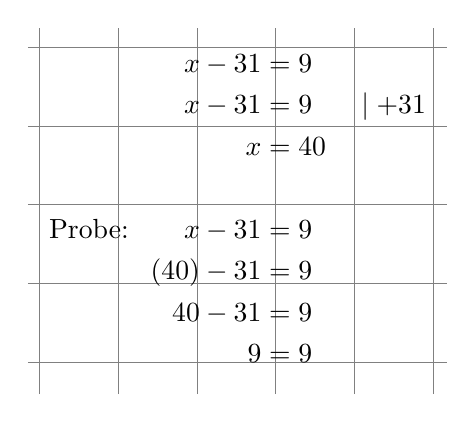
\begin{tikzpicture}[show background grid]
\node[below right] at (0,0.1) {
$\begin{aligned}
x-31  &= 9& &  \\
x - 31 &=9& & \mid + 31\\
x &=40& & 
\\
\\
\mbox{Probe:}\qquad x-31  &= 9& &  \\
\left(40\right)-31  &= 9& &  \\
40-31 &=9& &  \\
9 &=9& &  \\
\end{aligned}$};
\end{tikzpicture}
\endgroup
\\\hline
o)&\begingroup\setlength{\jot}{-0.03cm}
\tikzstyle{background grid}=[draw, black!15,step=.5cm]
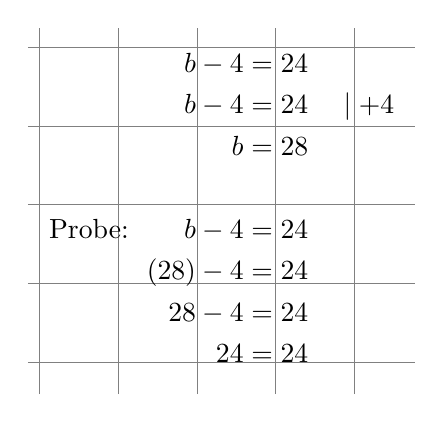
\begin{tikzpicture}[show background grid]
\node[below right] at (0,0.1) {
$\begin{aligned}
b-4  &= 24& &  \\
b - 4 &=24& & \mid + 4\\
b &=28& & 
\\
\\
\mbox{Probe:}\qquad b-4  &= 24& &  \\
\left(28\right)-4  &= 24& &  \\
28-4 &=24& &  \\
24 &=24& &  \\
\end{aligned}$};
\end{tikzpicture}
\endgroup
&
p)&\begingroup\setlength{\jot}{-0.03cm}
\tikzstyle{background grid}=[draw, black!15,step=.5cm]
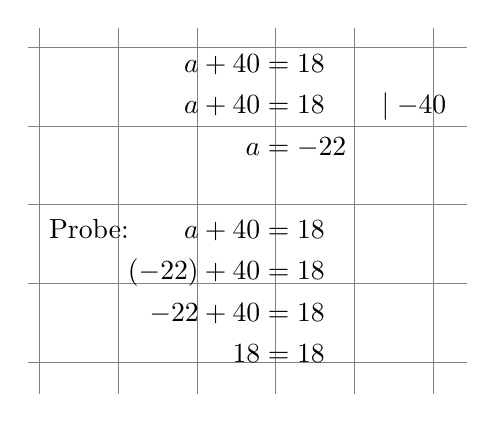
\begin{tikzpicture}[show background grid]
\node[below right] at (0,0.1) {
$\begin{aligned}
a+40  &= 18& &  \\
a + 40 &=18& & \mid - 40\\
a &=-22& & 
\\
\\
\mbox{Probe:}\qquad a+40  &= 18& &  \\
\left(-22\right)+40  &= 18& &  \\
-22+40 &=18& &  \\
18 &=18& &  \\
\end{aligned}$};
\end{tikzpicture}
\endgroup
\\\hline
q)&\begingroup\setlength{\jot}{-0.03cm}
\tikzstyle{background grid}=[draw, black!15,step=.5cm]
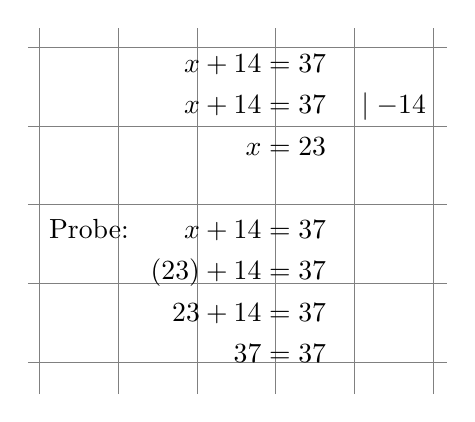
\begin{tikzpicture}[show background grid]
\node[below right] at (0,0.1) {
$\begin{aligned}
x+14  &= 37& &  \\
x + 14 &=37& & \mid - 14\\
x &=23& & 
\\
\\
\mbox{Probe:}\qquad x+14  &= 37& &  \\
\left(23\right)+14  &= 37& &  \\
23+14 &=37& &  \\
37 &=37& &  \\
\end{aligned}$};
\end{tikzpicture}
\endgroup
&
r)&\begingroup\setlength{\jot}{-0.03cm}
\tikzstyle{background grid}=[draw, black!15,step=.5cm]
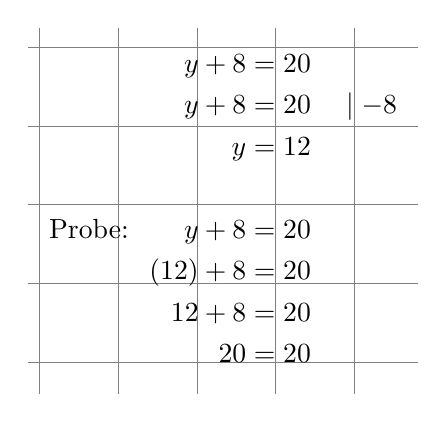
\begin{tikzpicture}[show background grid]
\node[below right] at (0,0.1) {
$\begin{aligned}
y+8  &= 20& &  \\
y + 8 &=20& & \mid - 8\\
y &=12& & 
\\
\\
\mbox{Probe:}\qquad y+8  &= 20& &  \\
\left(12\right)+8  &= 20& &  \\
12+8 &=20& &  \\
20 &=20& &  \\
\end{aligned}$};
\end{tikzpicture}
\endgroup
\\\hline
s)&\begingroup\setlength{\jot}{-0.03cm}
\tikzstyle{background grid}=[draw, black!15,step=.5cm]
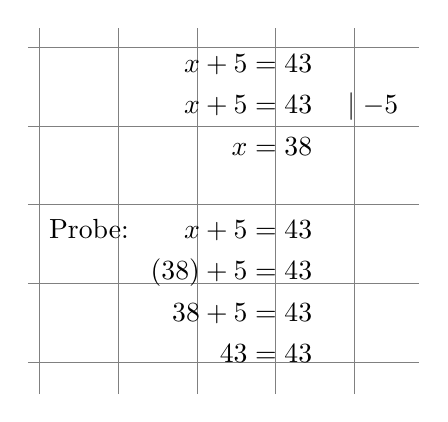
\begin{tikzpicture}[show background grid]
\node[below right] at (0,0.1) {
$\begin{aligned}
x+5  &= 43& &  \\
x + 5 &=43& & \mid - 5\\
x &=38& & 
\\
\\
\mbox{Probe:}\qquad x+5  &= 43& &  \\
\left(38\right)+5  &= 43& &  \\
38+5 &=43& &  \\
43 &=43& &  \\
\end{aligned}$};
\end{tikzpicture}
\endgroup
&
t)&\begingroup\setlength{\jot}{-0.03cm}
\tikzstyle{background grid}=[draw, black!15,step=.5cm]
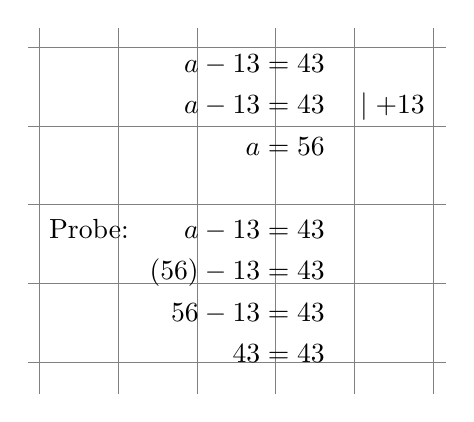
\begin{tikzpicture}[show background grid]
\node[below right] at (0,0.1) {
$\begin{aligned}
a-13  &= 43& &  \\
a - 13 &=43& & \mid + 13\\
a &=56& & 
\\
\\
\mbox{Probe:}\qquad a-13  &= 43& &  \\
\left(56\right)-13  &= 43& &  \\
56-13 &=43& &  \\
43 &=43& &  \\
\end{aligned}$};
\end{tikzpicture}
\endgroup
\\\hline
u)&\begingroup\setlength{\jot}{-0.03cm}
\tikzstyle{background grid}=[draw, black!15,step=.5cm]
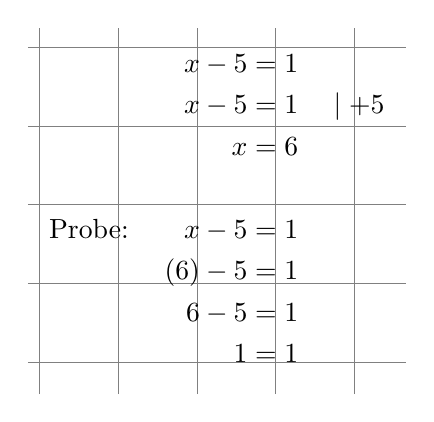
\begin{tikzpicture}[show background grid]
\node[below right] at (0,0.1) {
$\begin{aligned}
x-5  &= 1& &  \\
x - 5 &=1& & \mid + 5\\
x &=6& & 
\\
\\
\mbox{Probe:}\qquad x-5  &= 1& &  \\
\left(6\right)-5  &= 1& &  \\
6-5 &=1& &  \\
1 &=1& &  \\
\end{aligned}$};
\end{tikzpicture}
\endgroup
&
v)&\begingroup\setlength{\jot}{-0.03cm}
\tikzstyle{background grid}=[draw, black!15,step=.5cm]
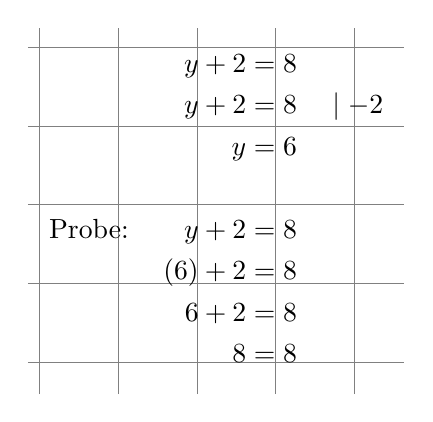
\begin{tikzpicture}[show background grid]
\node[below right] at (0,0.1) {
$\begin{aligned}
y+2  &= 8& &  \\
y + 2 &=8& & \mid - 2\\
y &=6& & 
\\
\\
\mbox{Probe:}\qquad y+2  &= 8& &  \\
\left(6\right)+2  &= 8& &  \\
6+2 &=8& &  \\
8 &=8& &  \\
\end{aligned}$};
\end{tikzpicture}
\endgroup
\\\hline
w)&\begingroup\setlength{\jot}{-0.03cm}
\tikzstyle{background grid}=[draw, black!15,step=.5cm]
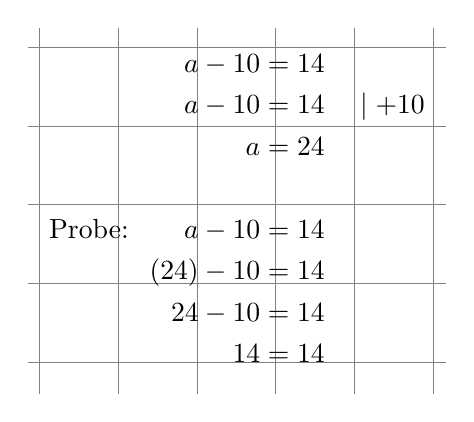
\begin{tikzpicture}[show background grid]
\node[below right] at (0,0.1) {
$\begin{aligned}
a-10  &= 14& &  \\
a - 10 &=14& & \mid + 10\\
a &=24& & 
\\
\\
\mbox{Probe:}\qquad a-10  &= 14& &  \\
\left(24\right)-10  &= 14& &  \\
24-10 &=14& &  \\
14 &=14& &  \\
\end{aligned}$};
\end{tikzpicture}
\endgroup
&
x)&\begingroup\setlength{\jot}{-0.03cm}
\tikzstyle{background grid}=[draw, black!15,step=.5cm]
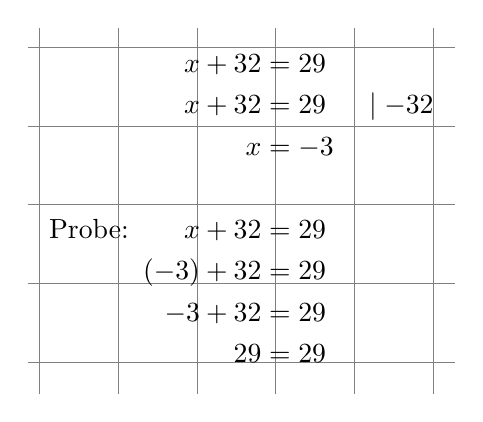
\begin{tikzpicture}[show background grid]
\node[below right] at (0,0.1) {
$\begin{aligned}
x+32  &= 29& &  \\
x + 32 &=29& & \mid - 32\\
x &=-3& & 
\\
\\
\mbox{Probe:}\qquad x+32  &= 29& &  \\
\left(-3\right)+32  &= 29& &  \\
-3+32 &=29& &  \\
29 &=29& &  \\
\end{aligned}$};
\end{tikzpicture}
\endgroup
\\\hline
y)&\begingroup\setlength{\jot}{-0.03cm}
\tikzstyle{background grid}=[draw, black!15,step=.5cm]
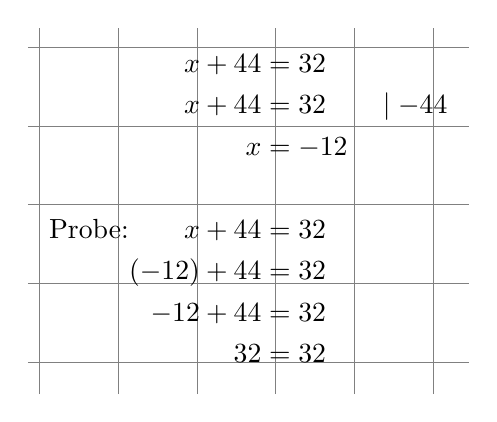
\begin{tikzpicture}[show background grid]
\node[below right] at (0,0.1) {
$\begin{aligned}
x+44  &= 32& &  \\
x + 44 &=32& & \mid - 44\\
x &=-12& & 
\\
\\
\mbox{Probe:}\qquad x+44  &= 32& &  \\
\left(-12\right)+44  &= 32& &  \\
-12+44 &=32& &  \\
32 &=32& &  \\
\end{aligned}$};
\end{tikzpicture}
\endgroup
&
z)&\begingroup\setlength{\jot}{-0.03cm}
\tikzstyle{background grid}=[draw, black!15,step=.5cm]
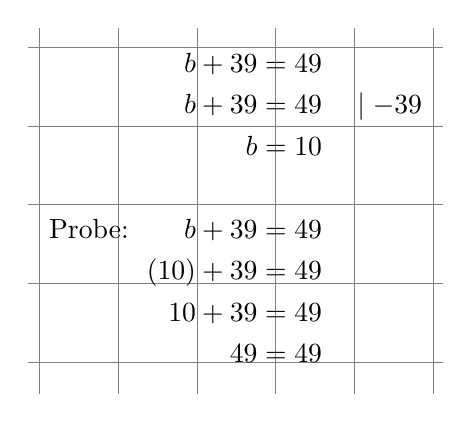
\begin{tikzpicture}[show background grid]
\node[below right] at (0,0.1) {
$\begin{aligned}
b+39  &= 49& &  \\
b + 39 &=49& & \mid - 39\\
b &=10& & 
\\
\\
\mbox{Probe:}\qquad b+39  &= 49& &  \\
\left(10\right)+39  &= 49& &  \\
10+39 &=49& &  \\
49 &=49& &  \\
\end{aligned}$};
\end{tikzpicture}
\endgroup
\\\hline
\end{xltabular}
\vspace{0.5cm}
\end{document}